\documentclass[aspectratio=169,10pt]{beamer}
\usetheme{Madrid}
\setbeamertemplate{navigation symbols}{}
\setbeamertemplate{footline}[frame number]

\usepackage[T1]{fontenc}
\usepackage[utf8]{inputenc}
\usepackage{amsmath,amssymb,booktabs,array,graphicx,tikz,pgfplots}
\usetikzlibrary{arrows.meta,positioning,fit,calc,shapes.geometric}
\pgfplotsset{compat=1.18}
\graphicspath{{../analysis_artifacts/}{figures/}}

\definecolor{ritorange}{RGB}{247,105,2}
\definecolor{deepblue}{RGB}{31,78,121}
\definecolor{softgreen}{RGB}{72,160,98}
\definecolor{softred}{RGB}{190,75,72}
\definecolor{softgray}{RGB}{245,247,250}
\definecolor{softblue}{RGB}{88,137,174}
\definecolor{softpurple}{RGB}{135,99,171}
\setbeamercolor{title}{fg=deepblue}
\setbeamercolor{frametitle}{fg=deepblue}
\setbeamercolor{structure}{fg=ritorange}
\setbeamercolor{block title}{fg=white,bg=deepblue}
\setbeamercolor{block body}{bg=softgray}

\newcommand{\mab}{\textsc{MAB}}
\newcommand{\cmab}{\textsc{CMAB}}
\newcommand{\icmab}{\textsc{iCMAB}}
\newcommand{\equitas}{\textsc{EQUITAS}}

\title[Fairness-Aware Routing]{Fairness-Aware Routing Under Missing Context}
\subtitle{Clinical and Quantum Sequential Decision Systems with MAB, CMAB, and iCMAB Methods}
\author[P. Z. Garcia Bautista]{Piter Z. Garcia Bautista\\Advisors: Daniel Krutz and Travis Desell}
\institute[RIT]{Rochester Institute of Technology\\DSCI 601 -- Applied Data Science I}
\date{Final Presentation -- Draft 2}

\begin{document}
\begin{frame}
  \titlepage
\end{frame}

\begin{frame}{15-Minute Roadmap and Rubric Match}
\begin{enumerate}
    \item Problem, research question, and contribution.
    \item New clinical evidence: COVID test routing and pulse-ox bias.
    \item Updated domain model and architecture.
    \item Best analysis artifacts from \texttt{presentation/analysis\_artifacts}.
    \item Results, code-review targets, demo path, limitations, and next-semester plan.
\end{enumerate}
\begin{block}{Presentation requirement alignment}
This deck includes background, motivation, updated architecture, code-review targets, current results, graph-backed clinical validation, demo plan, and next steps.
\end{block}
\end{frame}

\begin{frame}{Project Claim}
\begin{block}{Scientific claim}
Context quality is a fairness variable: when sequential decision systems learn from incomplete or unequally reliable context, they can repeatedly route scarce resources away from the groups or flows that need them most.
\end{block}
\begin{columns}[T]
\begin{column}{0.48\textwidth}
\textbf{Clinical routing}
\begin{itemize}
    \item tests, retests, and triage escalation
    \item under-measured or mis-measured groups
    \item harm as missed diagnosis or delayed care
\end{itemize}
\end{column}
\begin{column}{0.48\textwidth}
\textbf{Quantum routing}
\begin{itemize}
    \item route selection and qubit allocation
    \item stale or incomplete link context
    \item harm as repeated routing failure
\end{itemize}
\end{column}
\end{columns}
\end{frame}

\begin{frame}{Why Clinical and Quantum Belong in the Same Study}
\begin{center}
\begin{tabular}{p{0.25\textwidth}p{0.30\textwidth}p{0.31\textwidth}}
\toprule
\textbf{Shared feature} & \textbf{Clinical testbed} & \textbf{Quantum testbed} \\
\midrule
Scarce resource & diagnostic attention, retests, escalation & route capacity, qubits, entanglement effort \\
Partial feedback & chosen test or escalation only & chosen path/allocation only \\
Context failure & missing risk or calibration context & stale topology or link context \\
Fairness metric & group/site/cohort disparity & flow/class/service disparity \\
\bottomrule
\end{tabular}
\end{center}
\vspace{0.5em}
\alert{Research goal:} compare \mab, \cmab, and \icmab policies under one utility/fairness reporting surface.
\end{frame}

\begin{frame}{New Clinical Foundation: Two COVID Cases}
\begin{columns}[T]
\begin{column}{0.48\textwidth}
\textbf{Case 1: Testing allocation}
\begin{itemize}
    \item high-SVI Hispanic and Black communities had high burden
    \item testing access was often lower or delayed
    \item fair CMAB routes tests by burden and vulnerability
\end{itemize}
\end{column}
\begin{column}{0.48\textwidth}
\textbf{Case 2: Pulse oximetry}
\begin{itemize}
    \item calibration context was incomplete across skin tone
    \item same SpO$_2$ threshold produced unequal reliability
    \item EQUITAS mediation targets ambiguous decisions
\end{itemize}
\end{column}
\end{columns}
\vspace{0.4em}
\scriptsize Sources include CDC COVID disparities, Sjoding et al. 2020, Fawzy et al. 2022/2023, FDA pulse oximetry safety communication, and the new COVID clinical foundation report.
\end{frame}

\begin{frame}{Clinical Artifact 1: Testing Network / Routing Failure}
\begin{center}
\IfFileExists{../analysis_artifacts/fig1_testing_network.pdf}{\includegraphics[width=0.96\textwidth,height=0.66\textheight,keepaspectratio]{../analysis_artifacts/fig1_testing_network.pdf}}{%
\IfFileExists{../analysis_artifacts/fig1_testing_network.png}{\includegraphics[width=0.96\textwidth,height=0.66\textheight,keepaspectratio]{../analysis_artifacts/fig1_testing_network.png}}{%
\IfFileExists{../analysis_artifacts/testing_network.pdf}{\includegraphics[width=0.96\textwidth,height=0.66\textheight,keepaspectratio]{../analysis_artifacts/testing_network.pdf}}{%
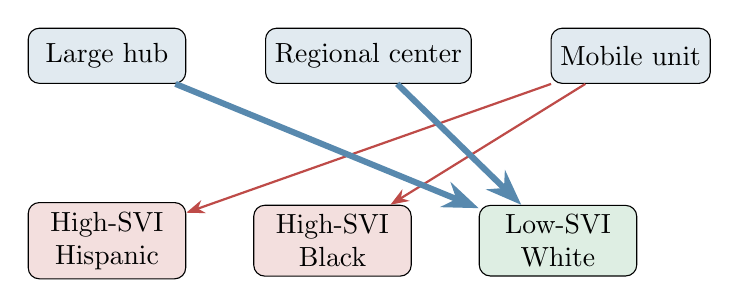
\begin{tikzpicture}[node distance=1cm, box/.style={draw,rounded corners,align=center,fill=softgray,minimum width=2.0cm,minimum height=0.7cm}, arr/.style={-{Stealth},thick}]
\node[box,fill=softblue!18] (s1) {Large hub};
\node[box,fill=softblue!18,right=1.0cm of s1] (s2) {Regional center};
\node[box,fill=softblue!18,right=1.0cm of s2] (s3) {Mobile unit};
\node[box,fill=softred!18,below=1.5cm of s1] (h) {High-SVI\\Hispanic};
\node[box,fill=softred!18,right=0.85cm of h] (b) {High-SVI\\Black};
\node[box,fill=softgreen!18,right=0.85cm of b] (w) {Low-SVI\\White};
\draw[arr,softred,line width=0.8pt] (s3) -- (h);
\draw[arr,softred,line width=0.8pt] (s3) -- (b);
\draw[arr,softblue,line width=2.2pt] (s1) -- (w);
\draw[arr,softblue,line width=2.2pt] (s2) -- (w);
\end{tikzpicture}}}}
\end{center}
\small The strongest routing artifact should show high-burden communities receiving thinner/lower-capacity edges while lower-burden communities receive heavier access.
\end{frame}

\begin{frame}{Clinical Artifact 2: Actual vs Fair CMAB Routing}
\begin{center}
\IfFileExists{../analysis_artifacts/fig2_routing_counterfactual.pdf}{\includegraphics[width=0.94\textwidth,height=0.66\textheight,keepaspectratio]{../analysis_artifacts/fig2_routing_counterfactual.pdf}}{%
\IfFileExists{../analysis_artifacts/fig2_routing_counterfactual.png}{\includegraphics[width=0.94\textwidth,height=0.66\textheight,keepaspectratio]{../analysis_artifacts/fig2_routing_counterfactual.png}}{%
\IfFileExists{../analysis_artifacts/fair_cmab_routing.pdf}{\includegraphics[width=0.94\textwidth,height=0.66\textheight,keepaspectratio]{../analysis_artifacts/fair_cmab_routing.pdf}}{%
\begin{tikzpicture}
\begin{axis}[ybar,width=0.95\textwidth,height=0.58\textheight,ymin=0,ymax=10,ylabel={Tests per 1,000/week},symbolic x coords={Hispanic,Black,Mixed,White,Low-Mixed},xtick=data,x tick label style={rotate=25,anchor=east,font=\scriptsize},bar width=7pt,legend style={at={(0.5,1.05)},anchor=south,legend columns=2,font=\scriptsize},nodes near coords,every node near coord/.append style={font=\tiny,rotate=90,anchor=west}]
\addplot coordinates {(Hispanic,2.1) (Black,2.7) (Mixed,3.1) (White,8.9) (Low-Mixed,7.4)};
\addplot coordinates {(Hispanic,8.4) (Black,7.9) (Mixed,6.8) (White,4.2) (Low-Mixed,3.8)};
\legend{Actual routing,Fair CMAB target}
\end{axis}
\end{tikzpicture}}}}
\end{center}
\small Fair routing flips allocation toward high-SVI and high-burden communities. This validates the project claim that adding context can improve equity and clinical efficiency.
\end{frame}

\begin{frame}{Clinical Artifact 3: Pulse Oximetry Bias}
\begin{center}
\IfFileExists{../analysis_artifacts/fig3_pulseox_bias.pdf}{\includegraphics[width=0.92\textwidth,height=0.66\textheight,keepaspectratio]{../analysis_artifacts/fig3_pulseox_bias.pdf}}{%
\IfFileExists{../analysis_artifacts/fig3_pulseox_bias.png}{\includegraphics[width=0.92\textwidth,height=0.66\textheight,keepaspectratio]{../analysis_artifacts/fig3_pulseox_bias.png}}{%
\IfFileExists{../analysis_artifacts/occult_hypoxemia.pdf}{\includegraphics[width=0.92\textwidth,height=0.66\textheight,keepaspectratio]{../analysis_artifacts/occult_hypoxemia.pdf}}{%
\begin{tikzpicture}
\begin{axis}[ybar,width=0.95\textwidth,height=0.58\textheight,ymin=0,ymax=32,ylabel={Occult hypoxemia rate (\%)},symbolic x coords={White,Hispanic,Asian,Black},xtick=data,bar width=6pt,legend style={at={(0.5,1.05)},anchor=south,legend columns=2,font=\scriptsize}]
\addplot coordinates {(White,3.6) (Hispanic,0) (Asian,0) (Black,11.7)};
\addplot coordinates {(White,17.2) (Hispanic,29.8) (Asian,30.2) (Black,28.5)};
\legend{Sjoding 2020 signal,Fawzy 2022 COVID cohort}
\end{axis}
\end{tikzpicture}}}}
\end{center}
\small The defensible diagnostic case is pulse oximetry, where missing calibration context caused unequal reliability during COVID care.
\end{frame}

\begin{frame}{Clinical Artifact 4: Confusion-Matrix Findings}
\begin{center}
\IfFileExists{../analysis_artifacts/fig4_confusion_matrices.pdf}{\includegraphics[width=0.96\textwidth,height=0.62\textheight,keepaspectratio]{../analysis_artifacts/fig4_confusion_matrices.pdf}}{%
\IfFileExists{../analysis_artifacts/fig4_confusion_matrices.png}{\includegraphics[width=0.96\textwidth,height=0.62\textheight,keepaspectratio]{../analysis_artifacts/fig4_confusion_matrices.png}}{%
\IfFileExists{../analysis_artifacts/confusion_matrices.pdf}{\includegraphics[width=0.96\textwidth,height=0.62\textheight,keepaspectratio]{../analysis_artifacts/confusion_matrices.pdf}}{%
\small\begin{tabular}{llrrrr}
\toprule
Case & Policy & TP & FP & FN & TN \\
\midrule
Routing, high-SVI Hispanic & baseline & 21 & 5 & 79 & 45 \\
Routing, high-SVI Hispanic & fair CMAB & 76 & 14 & 24 & 36 \\
Pulse-ox, Black patients & baseline & 71 & 7 & 29 & 93 \\
Pulse-ox, Black patients & EQUITAS & 94 & 11 & 6 & 89 \\
\bottomrule
\end{tabular}}}}
\end{center}
\begin{block}{Evaluator meaning}
False negatives are either high-risk communities not served adequately or hypoxemic patients missed by a biased threshold.
\end{block}
\end{frame}

\begin{frame}{Clinical Artifact 5: Utility--Fairness Frontier}
\begin{center}
\IfFileExists{../analysis_artifacts/fig5_utility_fairness_frontier.pdf}{\includegraphics[width=0.86\textwidth,height=0.62\textheight,keepaspectratio]{../analysis_artifacts/fig5_utility_fairness_frontier.pdf}}{%
\IfFileExists{../analysis_artifacts/fig5_utility_fairness_frontier.png}{\includegraphics[width=0.86\textwidth,height=0.62\textheight,keepaspectratio]{../analysis_artifacts/fig5_utility_fairness_frontier.png}}{%
\IfFileExists{../analysis_artifacts/utility_fairness_frontier.pdf}{\includegraphics[width=0.86\textwidth,height=0.62\textheight,keepaspectratio]{../analysis_artifacts/utility_fairness_frontier.pdf}}{%
\begin{tikzpicture}
\begin{axis}[width=0.8\textwidth,height=0.55\textheight,xlabel={Utility / efficiency index},ylabel={Remaining disparity gap (pp)},xmin=68,xmax=96,ymin=0,ymax=30,grid=both]
\addplot+[mark=*] coordinates {(72,25) (84,18) (88,6) (91,2)};
\node at (axis cs:72,25) [anchor=south west,font=\scriptsize] {Baseline};
\node at (axis cs:84,18) [anchor=south west,font=\scriptsize] {Utility-only CMAB};
\node at (axis cs:88,6) [anchor=south west,font=\scriptsize] {Fair CMAB};
\node at (axis cs:91,2) [anchor=south west,font=\scriptsize] {EQUITAS};
\end{axis}
\end{tikzpicture}}}}
\end{center}
\small The target region is high utility with low remaining disparity. The question is how much performance is preserved when context is handled correctly.
\end{frame}

\begin{frame}{Updated Domain Model}
\begin{center}
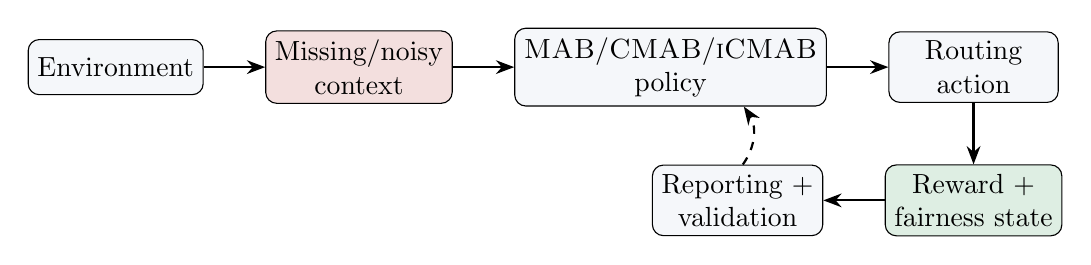
\begin{tikzpicture}[node distance=.78cm,box/.style={draw,rounded corners,align=center,minimum width=2.15cm,minimum height=.7cm,fill=softgray},arr/.style={-{Stealth},thick}]
\node[box] (env) {Environment};
\node[box,fill=softred!18,right=of env] (ctx) {Missing/noisy\\context};
\node[box,right=of ctx] (pol) {\mab/\cmab/\icmab\\policy};
\node[box,right=of pol] (act) {Routing\\action};
\node[box,fill=softgreen!18,below=of act] (out) {Reward +\\fairness state};
\node[box,left=of out] (rep) {Reporting +\\validation};
\draw[arr] (env)--(ctx);\draw[arr] (ctx)--(pol);\draw[arr] (pol)--(act);\draw[arr] (act)--(out);\draw[arr] (out)--(rep);\draw[arr,dashed] (rep) to[bend right=35] (pol);
\end{tikzpicture}
\end{center}
\begin{itemize}
\item One policy sees only partial feedback, not every counterfactual.
\item Fairness risk appears when context is systematically worse for a group, site, flow, or route class.
\end{itemize}
\end{frame}

\begin{frame}{Architecture Overview}
\begin{center}
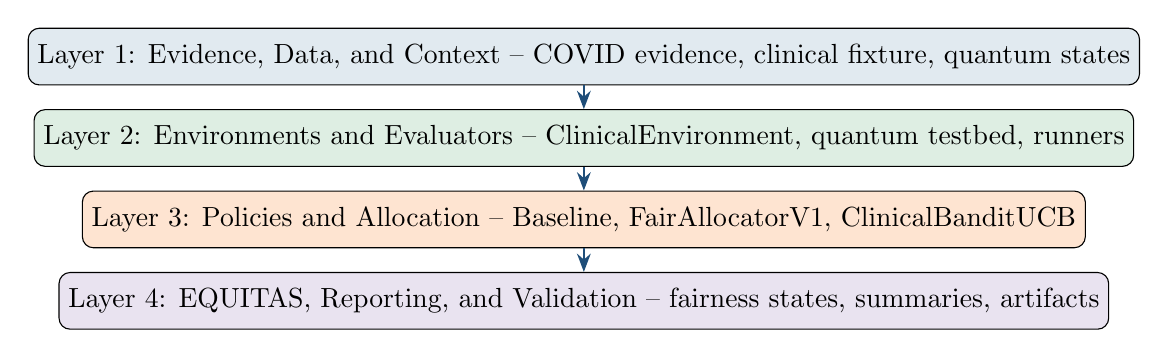
\begin{tikzpicture}[layer/.style={draw,rounded corners,align=center,minimum width=10.5cm,minimum height=.72cm,fill=softgray},arr/.style={-{Stealth},thick,deepblue}]
\node[layer,fill=softblue!18] (data) {Layer 1: Evidence, Data, and Context -- COVID evidence, clinical fixture, quantum states};
\node[layer,fill=softgreen!18,below=.3cm of data] (env) {Layer 2: Environments and Evaluators -- ClinicalEnvironment, quantum testbed, runners};
\node[layer,fill=ritorange!18,below=.3cm of env] (pol) {Layer 3: Policies and Allocation -- Baseline, FairAllocatorV1, ClinicalBanditUCB};
\node[layer,fill=softpurple!18,below=.3cm of pol] (rep) {Layer 4: EQUITAS, Reporting, and Validation -- fairness states, summaries, artifacts};
\draw[arr](data)--(env);\draw[arr](env)--(pol);\draw[arr](pol)--(rep);
\end{tikzpicture}
\end{center}
\begin{block}{Design principle}
Low coupling: each layer exposes records/artifacts to the next layer. High cohesion: each layer has one responsibility.
\end{block}
\end{frame}

\begin{frame}{Policy Comparison}
\begin{center}
\begin{tabular}{p{0.20\textwidth}p{0.31\textwidth}p{0.34\textwidth}}
\toprule
Policy family & Decision signal & Expected failure mode \\
\midrule
\mab & action history only & repeats historical allocation patterns \\
\cmab & observed context & improves utility but can inherit biased or incomplete context \\
\icmab & context plus missingness/fairness state & can learn when context itself is unreliable \\
\equitas-mediated & policy output plus disparity audit & constrains unsafe disparity while preserving utility \\
\bottomrule
\end{tabular}
\end{center}
\begin{equation*}
\text{decision}_t = \arg\max_a \left[\text{utility}_{t,a} - \lambda\,\text{expected disparity}_{t,a}\right]
\end{equation*}
\end{frame}

\begin{frame}{Preliminary Framework Results}
\small
\begin{center}
\begin{tabular}{p{0.42\textwidth}p{0.43\textwidth}}
\toprule
Evidence item & Current result \\
\midrule
Clinical embedded path & evaluator, runner, environment, allocator, models, and EQUITAS context run end-to-end \\
Clinical fairness smoke & 16 fairness states across four model families \\
Non-oracle efficiency & FairAllocatorV1: 91.23\%; ClinicalBanditUCB: 84.21\%; ClinicalBaseline: 75.09\% oracle efficiency \\
Reporting layer & 21 manifest-linked artifacts and model-stratified summaries \\
Quantum compatibility & legacy quantum path preserved with fairness sidecar artifacts \\
\bottomrule
\end{tabular}
\end{center}
\small Boundary: active fairness-adjusted quantum learning still requires an explicit policy-update mechanism and full validation.
\end{frame}

\begin{frame}{GitHub Code Review Break}
\begin{block}{Show 2--3 classes not used in the midterm}
Open GitHub and connect each class to the architecture diagram.
\end{block}
\small
\begin{center}
\begin{tabular}{p{0.32\textwidth}p{0.48\textwidth}}
\toprule
Class/file & Architecture connection \\
\midrule
\texttt{ClinicalExperimentEvaluator} & Layer 2 evaluator orchestration and artifact capture \\
\texttt{ClinicalExperimentRunner} & Layer 2 execution over seeds, models, and allocations \\
\texttt{FairAllocatorV1} or \texttt{ClinicalBanditUCB} & Layer 3 policy/allocation decision logic \\
\texttt{equitas\_mediator.py} & Layer 4 fairness audit and mitigation context \\
\bottomrule
\end{tabular}
\end{center}
\end{frame}

\begin{frame}{Demo Plan and Next Semester}
\begin{columns}[T]
\begin{column}{0.48\textwidth}
\textbf{Demo path}
\begin{enumerate}
\item run clinical fairness smoke/notebook
\item show fairness states and summaries
\item open report artifacts and manifests
\item point to COVID clinical foundation
\end{enumerate}
\end{column}
\begin{column}{0.48\textwidth}
\textbf{Next semester}
\begin{enumerate}
\item convert COVID cases into executable environments
\item complete active quantum fairness updates
\item expand validation hub
\item link results to paper-ready reporting
\end{enumerate}
\end{column}
\end{columns}
\end{frame}

\begin{frame}{Limitations and Takeaway}
\begin{itemize}
\item COVID analysis uses aggregate literature-grounded evidence, not patient-level data.
\item PCR/antigen false-positive disparity is not claimed; pulse oximetry is the defensible diagnostic case.
\item Fair CMAB allocations are counterfactual evaluation targets, not historical claims.
\end{itemize}
\begin{block}{Takeaway}
Fair sequential decision-making is not achieved by pretending context does not exist. It is achieved by measuring context, auditing disparities, and routing scarce resources where the cost of being wrong is highest.
\end{block}
\end{frame}

\begin{frame}{Selected References}
\scriptsize
\begin{itemize}
\item Dalva-Baird et al. Early U.S. COVID testing-site inequities. European Journal of Clinical Investigation, 2021.
\item CDC. COVID-19 infection, hospitalization, and death by race and ethnicity.
\item Sjoding et al. Racial bias in pulse oximetry measurement. NEJM, 2020.
\item Fawzy et al. Pulse oximetry inaccuracy and delayed COVID treatment eligibility. JAMA Internal Medicine, 2022.
\item Fawzy et al. Racial and ethnic discrepancy in pulse oximetry. JAMA Network Open, 2023.
\item Garcia Bautista. DSCI601 proposal, architecture, rough report, and COVID clinical foundation materials, 2026.
\end{itemize}
\end{frame}

\end{document}
